\documentclass[a4paper,11pt]{article}
%\documentclass{aa}
\usepackage{conference}
\usepackage{latexsym}
\usepackage[perpage,symbol*]{footmisc}
%\usepackage[utf8]{inputenc}
\usepackage[utf8x]{inputenc}
\usepackage{textcomp}
\usepackage[french]{babel}
\usepackage{amssymb,amsfonts,amsmath} % blackboard math symbols
\usepackage{graphicx}                 % graphics
\usepackage{cite}
\usepackage[varg]{txfonts}
\usepackage{booktabs}                 % professional-quality tables
\usepackage{tabularx}
\usepackage{enumerate}
%\usepackage{enumitem}
\usepackage{multicol}
%\usepackage[utf8]{inputenc}          % allow utf-8 input
\usepackage[T1]{fontenc}              % use 8-bit T1 fonts
\usepackage{hyperref}                 % hyperlinks
\usepackage{url}                      % simple URL typesetting
\usepackage{nicefrac}                 % compact symbols for 1/2, etc.
\usepackage{microtype}                % microtypography
%\usepackage[final]{graphicx}
\usepackage{tocloft}

\cftsetindents{section}{0em}{2em}
\cftsetindents{subsection}{0em}{2em}
\renewcommand\cfttoctitlefont{\hfill\Large\bfseries}
\renewcommand\cftaftertoctitle{\hfill\mbox{}}
\setcounter{tocdepth}{3}

%\begin{document}

\title{Retour vers le \emph{Cosmos}}
\author{
  F.M. Sanchez~hol137\thanks{Retired Professor} \\
  Department de physique\\
  Université Paris 11 Orsay \\
  Paris, FRANCE \\
  \texttt{hol137-at-yahoo.fr} \\
  %% examples of more authors
   \And
 M.H. Grosmann\thanks{Retired Professor} \\
  Department de photonique\\
  Université de Strasbourg\\
  Strasbourg, FRANCE \\
  \texttt{michel.grosmann-at-me.com} \\
   \And
 D. Tassot\thanks{Retired Professor} \\
  Ecole des Mines\\
  %University of Strasbourg\\
  %Strasbourg, FRANCE \\
  \texttt{d.tassot-at-me.com} \\
   \And
 C. Bizouard\thanks{Astronome} \\
  Observatoire de Paris\\
  Paris, FRANCE \\
  %
  %\texttt{c.bizouard-at-me.com} \\
  %% Coauthor \\
  %% Affiliation \\
  %% Address \\
  %% \texttt{email} \\
  %% \And
  %% Coauthor \\
  %% Affiliation \\
  %% Address \\
  %% \texttt{email} \\
  %% \And
  %% Coauthor \\
  %% Affiliation \\
  %% Address \\
  %% \texttt{email} \\
}


\begin{document}
\maketitle

%\{tableofcontents}
\tableofcontents
\clearpage
% keywords can be removed
\keywords{Quantum \and Holography \and Cosmos}

\section*{Introduction}
\addcontentsline{toc}{section}{Introduction}

%\section{Introduction}

Le modèle dit du Big-Bang est une description de l'origine et de l'évolution de l’Univers datant du début du 20éme siècle.

De façon générale, le terme « Big Bang » est associé à toutes les théories qui décrivent notre Univers comme issu d'une dilatation rapide. Par extension, il est également associé à cette époque dense et chaude qu’aurait connue l’Univers il y a 13,8 milliards d’années, (sans que cela préjuge forcément de l’existence d’un « instant initial » ou d’un commencement à son histoire).

\subsection{Le modèle du ”Big-Bang”}
\label{sec:headings}

Le terme a été initialement proposé en 1927 par l'astrophysicien  et chanoine catholique belge Georges Lemaître, qui décrivait dans les grandes lignes l’expansion de l'Univers, plus précisément décrite par l'astronome américain Edwin Hubble en 1929. Ce modèle fut désigné pour la première fois sous le terme ironique de « Big Bang » lors d’une émission de la BBC, The Nature of Things en 1949 (dont le texte fut publié en 1950), par le physicien britannique Fred Hoyle. Lui-même préférait les modèles d'état stationnaire.

%Voir Section \ref{sec:headings}.

\subsubsection{Concept General}
%\lipsum[5]
Le concept général du Big Bang, à savoir que l’Univers est en expansion et a été plus dense et plus chaud par le passé, doit sans doute être attribué au Russe Alexandre Friedmann, qui l'avait proposé en 1922, cinq ans avant Lemaître. Son assise fut cependant considérée comme mieux établie en 1965 avec la découverte du fond diffus cosmologique. Georges Lemaître le qualifia d’« éclat disparu de la formation des mondes, attestant de façon définitive la réalité de l’époque dense et chaude de l’Univers primordial ». Albert Einstein, en mettant au point la relativité générale, aurait pu déduire l'expansion de l'Univers, mais a préféré modifier ses équations en y ajoutant sa constante cosmologique, car il était persuadé que l'Univers devait être statique.

Le terme de « Big Bang chaud » (« Hot Big Bang ») est parfois utilisé initialement pour indiquer que, selon ce modèle, l’Univers était plus chaud quand il était plus dense.

\subsubsection{Partisans et adversaires: la controverse}

Partisans et adversaires du modèle du Big Bang.

Dès le début, ce modèle fut jugé séduisant par tous les amateurs d'un concept de « création » de l'Univers. Mais les tenants de l'énoncé attribué à Lavoisier : « Rien ne se perd, rien ne se crée ! Tout se transforme ! », réagirent dès le début négativement à la proposition. 

Par ailleurs de grandes critiques furent présentées sur les évaluations numériques de l'espace et du temps aux grandes distances envisagées : Dans ce modèle, les mesures de temps et d'espaces sont les unes et les autres basées sur le « décalage spectral » dû à l'effet Doppler. Dans le principe ceci ressemble à la mesure par les radars de la police de la vitesse des véhicules : 

Si un objet vibrant à une fréquence f1 s'éloigne de nous avec une vitesse V, nous le percevons (à cause de la vitesse limitée de la lumière) comme vibrant avec une fréquence f2 plus petite, (on dit «  décalée vers le rouge »). La mesure de la différence $Df = f1 – f2$ permet d'évaluer la « vitesse d'éloignement » de l'objet par rapport à l'observateur. 

Pour les « objets célestes » proches de nous on peut mesurer les positions et les vitesses par triangulation. Des mesures expérimentales permirent de comparer les valeurs de distances et vitesses obtenues par triangulation et les valeurs de «  décalage spectraux ». Hubble et Humason constatèrent une proportionnalité entre les valeurs des positions et des vitesses et présentèrent cette proportionnalité (« Lois de Hubble ») comme une observation expérimentale. Mais cette proportionnalité découle naturellement du fait que ces valeurs sont respectivement obtenues en multipliant le décalage Df par un coefficient A pour la première et B pour la seconde ! Elle est donc simplement le quotient de A par B !

Pour les objets célestes trop éloignés pour permettre des mesures géométriques des distances et des vitesses une autre méthode d'évaluation fut découverte : des objets célestes, les « céphéides » présentent une luminosité qui varie périodiquement. La mesure de la fréquence correspondante permet une « autre évaluation » de la distance et de la vitesse. Elle semble confirmer le modèle du BIG-BANG.

Mais elle est aussi basée sur le principe de l'effet Doppler. Et a le même défaut que la première : Il est bien difficile de discriminer entre « décalage dû à un déplacement longitudinal » et « décalage dû à un déplacement transversal ».

Les partisans du BIG-BANG expliquent qu'il n'y a « que des déplacements longitudinaux ».

Leurs adversaires rétorquent que « justement cela reste à démontrer » et que les données expérimentales permettent d'envisager une « Univers en rotation » aussi bien qu'un « Univers en expansion » …

Depuis bientôt un siècle, les controverses ne font que s'amplifier. La Science-Fiction a inspiré de nouvelles idées et concepts sur les « temps » et les « espaces » : virtualités, multivers, trous de vers, etc …

\subsection{Le ”modèle Cosmologique"}
\label{sec:headings}

Dans ce modèle il n'y a pas de « début » ni de « fin » de l'Univers.

D'une part il est vraisemblable que le développement des techniques expérimentales et de l'amélioration corrélative des théories en optique (LASERs, Optiques Holographiques, Photonique, etc… ) va peut-être prochainement permettre de très grandes améliorations en observations. De nouvelles données expérimentale sont recueillies tous les jours par quantité d'instruments qui n'existaient pas il y a quelques années

D'autre part des considérations théoriques nouvelles essaient de prendre en compte ces nouveaux résultats. Les unes pour les intégrer dans des théories existantes. D'autres pour servir de bases à de nouvelles théories. 

Le ”modèle Cosmologique” (développé par l’équipe du professeur Francis M. Sanchez) en est un exemple : Il suppose un Univers Visible limité par la vitesse de la lumière mais intégré dans un Univers plus vaste. 

On peut faire l'analogie avec une taupinière, au sommet de laquelle des taupes très myope et qui ne voient pas jusqu'à la base de la taupinière, ont imaginé un Univers limité au sommet de leur taupinière. Mais qui, développant des instruments, leur permettant d'agrandir leur champ de vision, découvrent petit à petit, qu'au bas de la taupinière existent peut-être des « choses » (terre, brins d'herbe etc …) qu'elles essaient de se représenter … en polémiquant entre elle sur les différents « modèles » possibles …

En appliquant les principes de la thermodynamique (qui font déjà polémiques au niveau de la planète et du réchauffement climatique) à l'Univers, il est possible d'imaginer un Univers cyclique de très grandes dimensions.

Il serait composée de deux parties : l'une visible ”tardionique” à « courte » portée … L'autre « tachyonique » à bien plus grande échelle !

Ce modèle permet de réconcilier les contradictions entre MACRO- et micro- Physiques et évite les paradoxes de « matière noire et « énergie noire » qui handicapent les modèles de type Big-Bang …

Certaines vérifications expérimentales pourront être prochainement effectuées par des satellites en projet et par des expériences, lors du redémarrage dans 2 ans du CERN à Genève.


\section{Le concept de Cosmos à travers les ages}


\section{Le testament de Pythagore}



\section{Le désenchantement des sciences modernes}


\subsection{La Science, cette inconnue}

L'incompréhension générale de ce qu'est réellement la Science est illustrée par la célèbre formule d'Einstein "le plus incompréhensible est que le Monde soit compréhensible". Car la Science, qui se confondait jadis avec la Philosophie, terme forgé par Pythagore, le premier véritable homme de Science,  était unifiée, contrairement à l'actuelle éclatement des sciences, et concerne au premier chef le Monde, c'est-à-dire le Cosmos, la préoccupation centrale de Pythagore.

Donc, fondamentalement, la Science, ou Philosophie Naturelle, est la connaissance et compréhension du Cosmos, ce qui signifie sémantiquement un Univers bien ordonné. Noter que la cosmologie officielle définit l'Univers comme 'un ensemble de particules en interaction', donc régies par certaines lois. Mais il ne suffit pas qu'il y ait des lois, encore faut-il qu'elles soient bonnes, c'est-à-dire esthétiques,  acceptables par l'esprit humain. Il faut donc répondre à Einstein:

\textit {Le plus compréhensible, c'est que l'humain soit cosmique}

Cela implique que seule la connaissance du Cosmos peut expliquer ce qu'est l'humain et la Science. Pour cette raison, certains ont traité l'humain "d'animal cosmique", et introduisent une "conscience cosmique". En particulier, l'hypothèse d'un Cosmos calculateur implique que l'humain soit aussi calculateur, ce qui explique son attrait pour les nombres et l'harmonie musicale, liaison prêtée à Pythagore, qui, plus généralement, affirmait que tout est nombre. Mais Pythagore ne considérait que des nombres entiers : il anticipait ainsi la Physique Quantique.  

Celle-ci s'est imposée d'abord par l'observation des cristaux manifestant des formes géométriques spectaculaires, puis par la "loi des proportions définies" qui régit le nombre d' atomes composant une molécule. Le plus souvent ces rapports sont simples, ainsi l'eau se compose de 2 parties d' Hydrogène pour 1 partie d'Oxygène. Les nombres entiers sont aussi apparus dans les longueurs d'onde spectrales, puis dans les interactions lumière-matière (Planck-Poincaré). A ce sujet l'intervention de Poincaré fut décisive, car Planck ne pouvait admettre une telle quantification.

D'où venait cette réticence de Planck ? C'est que Pythagore avait été oublié, comme montré dans le chapitre précédent, et les formalistes avaient voulus prendre le pouvoir. Les mathématiciens s'étaient séparés en trois groupes, les intuitionnistes, les formalistes et les logiciens. Les premiers, comme Poincaré, veulent rester en contact avec le Monde. Mais les formalistes, tel Hilbert, veulent tout axiomatiser à partir de l'Arithmétique. C'est ainsi que son sixième problème à résoudre parmi les 23 du millénium de 1900 était "d'axiomatiser la physique". On voit l'audace outrancière d'une telle proposition. 

Quant aux logiciens, ils voulaient pousser l'axiomatisation à son extrême, en démontrant l'Arithmétique elle-même. C'est ainsi que Bertrand Russell, dans son "Acta Mathematica" démontra 1 + 1 = 2, après 180 pages. Il est significatif que ce soit un soi-disant "philosophe" qui se soit livré à un si grotesque exercice. Cela illustre le fait que les philosophes modernes ont détesté les nombres entiers de Pythagore. Le ridicule de la situation fut dénoncé plus tard par le "théorème d'incomplétude" de Gödel. Il fut suivi par les informaticiens Turing et Von Neumann qui établirent "un théorème d'indécidabilité". 

Mais cela ne découragea pas les formalistes et les logiciens, qui finirent par vouloir introduire le formalisme dans l'enseignement des mathématiques modernes, avec les conséquences désastreusess que l'on sait. 

De plus, Von Neumann osa même proposer un "théorème de complétude de la Théorie Quantique", qui fit autorité, avant d'être réfuté, mais seulement beaucoup plus tard, par David Bohm. C'était un rejet total du Cosmos, en ce sens que le hasard est censé intervenir en microphysique. Cela s'appuyait sur le principe d'indétermination de Heisenberg, qui n'était en fait qu'une simple application de la complémentarité onde-particule, le concept le plus troublant, et incompris, de la physique moderne.

Le célèbre professeur Feynman, après avoir avoué dans ses célèbres cours de physique que personne ne comprenait rien à la physique quantique, aurait avancé la phrase décisive suivante : la lumière se propage par onde mais se réceptionne par quanta. Malheureusement, il ne tira pas de cela la leçon assez évidente suivante: la propagation par onde concerne l'Espace Cosmique, car l'onde est la propension à envahir tout l'espace disponible, tandis que la réception quantique est l'apanage d'une sélection cosmique calculatoire spatio-temporelle ultra-précise qui veut que toute l'énergie, au départ concentrée sur un seul atome, se retrouve en final, intégralement, sur un autre. On ne peut qu'apprécier l'extrême beauté, ce sens annexe du mot cosmos, de cette complémentarité Cosmos-Atome. 

Einstein eut été bien inspiré d'approfondir cette liaison Cosmos-Atome, comme on le verra plus loin. Il eut le mérite de s'opposer au hasard quantique quand il déclara "Dieu ne joue pas aux dés". Mais il eut le tort d'introduire le concept de "photon libre". Il le reconnut implicitement quand il déclara 'si on vous dit avoir compris le photon, vous répondrez que c'est mensonge".

Généralisant la phrase ci-dessus de Feynman, on en déduit que tout se propage par onde, y compris la matière. Avec pour conséquence que chaque objet est construit et déconstruit en permanence, dans une oscillation très rapide. Autrement dit le Big Bang est permanent. La symétrie matière-antimatière s'interprète alors par une oscillation entre matière et antimatière. 

Ainsi chacun est le centre d'une bulle "Univers" qui le construit et le déconstruit en permanence. Le Cosmos se présente donc comme disait Pascal: une sphère dont le centre est partout et la circonférence nulle part.

De plus, en introduisant un sens de rotation précis lors du balayage universel de reconstruction, cela introduit la "violation de la parité", c'est-à-dire la dissymétrie droite-gauche des réactions entre particules. 

A noter qu'on retrouve cette chiralité dans les molécules biologiques. Un sucre "inversé", c'est-à-dire qui a une orientation différente dans l'agencement de ses atomes, apparaît lors des synthèses chimiques, mais n'a aucun goût, ni aucune action biologique. Le fait que toute vie sur terre correspond au même ADN et avec la même orientation exclut l'intervention du hasard en biologie. En effet si le hasard jouait, la vie serait apparue plusieurs fois, avec les deux orientations possibles.

Cette oscillation matière-antimatière ouvre la porte à une explication simple de la mystérieuse "matière noire" qui constitue 25 \% de l'Univers. Ce serait une oscillation en quadrature, donc incapable de réagir avec la matière ordinaire. 


\subsection{Le carcan du réductionnisme moderne}

    Mais la Science a été trahie de façon encore plus profonde que ces divagations des formalistes et logiciens: on a systématiquement remplacé le raisonnement holistique naturel par le "réductionnisme". Au lieu d'expliquer les parties par le tout, on a prétendu expliquer le tout par les parties. C'est l'origine de l'éclatement de la Science en plusieurs disciplines officielles.

     En particulier, la Biologie s'est trouvée séparée car s'il est relativement facile de comprendre que chez l'être vivant les parties sont ordonnées au tout, les soi-disant scientifiques contemporains pensent qu'il n'en est rien dans le monde inerte. 

    Comme échappatoire, on invoque le concept d'"émergence" pour dire que "le tout est supérieur à l'addition de ses parties". Bien entendu, il faut introduire au contraire le "principe d'immergence", selon lequel, le tout explique l'agencement des parties. 

    Il est significatif que ce terme d'immergence soit un parfait néologisme. Autrement dit, le concept de Cosmos a été éradiqué de la pensée commune depuis longtemps. On peut attribuer l'origine de cette déviation au siècle des soi-disant "lumières" où Descartes, en particulier, cherchait à expliquer le mouvement des astres par des tourbillons d'éther faisant avancer les planètes dans le même sens. Hélas pour lui, on s'aperçut que certaines comètes avaient un mouvement rétrograde.


\subsection{Les principes holistiques}

Pour résoudre une question de physique il y a deux types de méthodes. L'une, réductionniste, consiste à étudier chaque détail dans un déroulement temporel. L'autre, holistique, invoque des principes généraux de conservation.

Le principe de la conservation d'énergie est le plus connu. L'énergie apparaît comme la monnaie d'échange universelle dans les interactions. Le simple fait que l'énergie ne peut être créée, mais seulement être transformée, selon le mot de Lavoisier, qui s'applique particulièrement bien à l'énergie : "Rien ne se perd, rien ne se crée, tout se transforme", montre que le Cosmos est un calculateur.  En effet, on voit mal comment une ménagère pourrait équilibrer son budget mensuel sans calculer.

La fameuse énergie sombre, qui constituerait 70 \% de l'énergie dans l'Univers, n'est qu'un faux problème, car les formules élémentaires de la physique de niveau bac montrent que l'énergie gravitationnelle de l'Univers n'est que 30\% de l'énergie totale (note N.3.1). 

La grande majorité des cosmologues a suivi la première méthode réductionniste, en partant d'équations locales pour en espérer déduire le tout. Voila l'origine des problèmes terribles qu'ils rencontrent actuellement, détaillés chapitre 5. Par contre une minorité a voulu établir la cosmologie sur des grands principes, en particulier le Principe Cosmologique Parfait, qui veut que l'Univers est partout le même et en tout temps. C'est cette dernière condition temporelle, qui lui vaut l'adjectif de "parfait" qui fait toute la différence entre cette cosmologie stationnaire et la cosmologie officielle. Pour cette dernière il y a eu un Big Bang initial. Comme suggéré plus haut il faut le remplacer par un Big Bang permanent, ce qui sera prouvé par le principe holistique le plus simple, le Principe Holographique.

 Le Principe Holographique décrit la conservation de l'information dans un Cosmos parfaitement ordonné. L'exemple le plus simple s'applique à un disque de rayon unité : sa circonférence est le double de son aire, ce qui est le testament qu'Archimède a fait inscrire sur sa tombe. La note 3.2 rappelle comment ce simple facteur 2 est le même que celui qui figure dans l'énergie cinétique élémentaire, et la relation critique d'un trou noir.

La forme diophantienne, c'est-à-dire purement arithmétique, du Principe Holographique est le Principe Holique, dont le représentant le plus simple est la 3ième loi de Képler, qu'il mis 10 ans après avoir trouvé les 2 premières (la forme elliptique et la loi des aires), à savoir la proportionnalité du cube des rayons avec le carré des périodes. La note 3.3 montre que la symétrie entre les constantes cosmiques G et h définies ci-dessous conduit à l'Univers critique.

\subsection{Les constantes cosmiques et l'Univers d'Eddington}

Newton avait l'esprit cosmique, contrairement au réductionniste Descartes. C'est ainsi qu'il chercha un lien entre la chute d'une pomme et le mouvement de la lune. Il introduisit donc G, la première 'constante cosmique" appelée couramment "constante universelle", ce qui signifie que c'est une grandeur physique mesurable invariante en tout lieu et en tout temps. 

On rejoint alors le concept de la Permanence Cosmique de Parménide, qui contredisait Héraclite d'Elée, pour qui "rien n'est constant sauf le mouvement". Bien au contraire, la vraie Science  redémarrait avec cette constante cosmique permanente. Surtout que d'autres constante cosmiques allaient suivre, comme la fameuse constante de Planck ci-dessus. Contrairement à l'affirmation courante, réductionniste, qui veut que cette constante ne s'applique qu'en micro-physique, cette constante de Planck est absolument essentielle au niveau cosmique. Par exemple, elle apparaît déjà dans le calcul du rayon d'une étoile.

Les observations astronomiques ont permis de mesurer la vitesse-lumière, troisième constante cosmique. Il a suffit d'observer les satellites de Jupiter pour constater une déviation progressive pendant 6 mois, qui se compense pendant les 6 mois suivants, donc manifestement due au mouvement de la Terre, et à une vitesse finie de la lumière. Grâce à l'arpentage du système solaire réalisé par l'Académie de Paris, à partir de la distance Terre-Mars, obtenue par parallaxe stellaire dans une mission en Guyane, on put en inférer la distance Terre-Jupiter, et ainsi Roemer put en déduire c, à l'observatoire de Paris On se rendit compte qu'elle était beaucoup trop rapide pour pouvoir être mesurée par des moyens terrestres. Mais, par contre, elle s'avéra très lente dès qu'on aborde les distances cosmiques. Ceci est d'une importance cruciale: l'opinion commune qui veut que la vitesse c soit une vitesse limite est contradictoire avec un Cosmos bien ordonné, qui nécessite au contraire des vitesses d'interaction très rapides.

Rappelons que, en toute rigueur, la théorie de la Relativité de Poincaré autorise deux domaines : l'un, le monde ordinaire, est peuplé de bradyons, dont la vitesse limite est effectivement c. L'autre est peuplé de tachyons dont c est, au contraire, la vitesse limite inférieure. La constante cosmique c est donc une frontière entre deux domaines. Beaucoup nient l'existence de ces tachyons, mais une observation confirme leur existence : l' oscillation non-Doppler dans les quasars. C'est un effet qui n'est pas considéré comme 'réaliste' par les officiels, car il contredit le dogme officiel qui nie l'existence des tachyons, donc cette oscillation cosmique n'est pas vérifiée, faute de crédits (voir le chapitre 7 qui détaille les procédures ineptes du système scientifique officiel).

\subsection{Le Principe Conceptuel}
 

Dans les 30\% d'énergie cosmique effective ci-dessus, le nombre d'atomes d'Hydrogène, a été prédit correctement par Eddington dans une formule très élégante et simple, précise au millième près, rappelée dans la note 3.4. De plus son interprétation statistique de la corrélation des grands nombres conduit à une autre formule du rayon critique de l'Univers, qui, précisément, ne dépend pas de c. Le rapprochement des deux méthodes conduit à une valeur de G au milliardième (Annexe 2).

Le point essentiel est que la formule du rayon d'Eddington est du même type que celle de l'atome, apparaissant comme une élimination de c entre la longueur d'onde de l'électron et le rapport de force quantique-gravitation. Le rapport du rayon de l'atome à cette longueur d'onde de l 'électron est la constante électrique $a \approx 137.0359991$ (voir ch. 4).
  
Mais Eddington, pourtant d'abord reconnu comme étant le meilleur théoricien de l'époque, a été unanimement rejeté par ses soi-disant "pairs" (sauf Schrödinger, le plus lucide des pères fondateurs classiques). Il faut reconnaître que sa Fundamental Theory est très difficile à comprendre, même pour des spécialistes comme Schrödinger. 


Mais surtout, dans le contexte réductionniste ambiant, on ne pouvait imaginer que la cosmologie puisse être aussi simple. On a invoqué que la sénilité d'Eddington était responsable de son net glissement vers un traitement pythagoricien de la physique.

C’est une sorte de miracle qu’à partir des considérations complexes, utilisant des mathématiques de haute volée qu’on peut tirer des formules finales d’ Eddington une image simple et claire de l’univers (note N.3.5). C’est la claire manifestation du Principe Conceptuel qui fonde la Science.



\subsection{Le Cosmos anthropique}

A partir des trois constantes cosmiques ci-dessus, G, $\hbar$ et c on peut calculer trois quantités fondamentales, qu'on appelle les unités de Planck. La masse de Planck, 22 ng a une interprétation directe claire, mas signalée nulle part : elle est voisine de la masse de la plus grosse cellule humaine, l'ovocyte. Par contre, la longueur et le temps de Planck sont beaucoup trop petits pour avoir une interprétation directe, mais interviennent de façon décisive dans les relations holographiques gouvernant l'Univers critique (note N.3.6). 

Noter qu'une autre circonstance vient brouiller encore plus cette Science cosmique si claire. On a osé introduire un système d'unités international faisant intervenir 7 grandeurs fondamentales, grotesque déviation détaillée dans l'annexe 1. 

La conscience humaine ayant retrouvé, grâce à la cette possibilité d’interpréter simplement les résultats Eddington, une place centrale dans le Cosmos, qu'en est-il des autres constantes biologiques ?

D'après le livre prophétique de Shrödinger "Qu'est-ce que la vie?", qui annonçait la biologie moléculaire, une caractéristique biologique essentielle est la température, élément essentiel des mutations. En effet, l'ours polaire et l'antilope africaine ont la même température, ce qui est, à priori, un gâchis terrible d'énergie. Il faut donc que l'impératif de mutation soit primordial.

En introduisant les longueurs d'onde de l'électron et de l'Hydrogène, le principe holographique définit la température de l'Univers (note 3.7). En la comparant à la température des mammifères, on obtient le facteur d'échelle, correspondant à $37.2^{\circ}$C, qui est lié au rayon d'une cellule, elle-même moyenne entre le rayon de l'Univers et la longueur de Planck ci-dessus. 

    Par ailleurs nous avons détecté dans l'ADN la présence manifeste des constantes principales de la physique. Par exemple la masse moyenne des quatre nucléotides A,T,G,C est voisine de la masse de Fermi, si importante en physique de particules. Les couples AT et GC ayant pratiquement la même masse, la masse du codon complet, comportant 6 nucléotides, est bien définie, et est voisine de 1837 fois la masse d'un atome d'Hydrogène, lui-même 1837 fois la masse d'un électron. Personne n’a signalé ce fait essentiel, car il prouve le caractèe universel de la vie. On voit sur cet exemple combien est néfaste la séparation entre les disciplines, les biologistes n’ayant vu aucun intérêt à considérer la masse atomique des nucléotides.

    De plus cette masse du bi-codon s'inscrit dans l'analyse tachyonique de la période non-Doppler des quasars (note 6). Donc les codons de l'ADN sont en connexion avec l'horloge cosmique absolue. Rappelons que tout ordinateur s'appuie sur une horloge. D'où la proposition que l'hélice d'ADN soit un hologramme-ligne. La prédiction qu'elle est effectivement parcourue par un courant électrique a été confirmée récemment. Du coup, les découvertes de Benvéniste sur la mémoire de l'eau reposent sur une base solide  (chapitre 6).

La vie est donc bien un phénomène cosmique. Par ces correspondances, la vie trouve une place centrale dans l'Univers. 

A noter que les officiels ont introduit un "principe anthropique" qu'ils ont utilisé à contre-sens, prétendant que le Cosmos servait l’humain. En fait, il est plus logique de considérer que le Cosmos calculateur se dote de  "périphériques" pour accompagner ses calculs. 


\subsection{Le demi-rayon critique d'Univers en 3 minutes}

     L'université d'Orsay a octroyé une année sabbatique 1997-98 au professeur d'holographie Sanchez pour qu'il présente deux rapports sur l'application du principe holographique à la physique théorique. Dans ses trois premières minutes, il a appliqué ce qu'il enseigne à ses étudiants : tout domaine doit d'abord s'appuyer sur les trois constantes universelles les plus adaptées au domaine considéré. En cosmologie, il faut donc remplacer c, vitesse beaucoup trop lente, par une autre constante universelle. Le plus immédiat est la masse moyenne de l'électron, du proton et du neutron, les trois particules principales de la physique atomique, ce qui revient à la formule d'Eddington ci-dessus, puisque les masses du proton et du neutron sont voisines. 

Le demi-rayon critique de l'Univers, donc sa masse, ont été ainsi obtenu en trois minutes d’un calcul élémentaire obligatoire, que personne n’a fait pendant un siècle.

Quelques semaines après, "l'holographie toponique" (Note 3.10) était mise en évidence, et devant le refus de l'Université d'Orsay de prendre l'article correspondant au sérieux "L' Univers conserve-t-il l'information ?", il fut mis sous pli cacheté en Mars 1998 à l'Académie des sciences. Le doyen d'Orsay, Jean-Claude Roynette, s'est basé sur une expertise anonyme négative, dont une indiscrétion fait penser qu'il s'agit de Jean-Jacques Lévy-Leblond (annexe 3). 


\subsection{Notes du chapitre 4}
 
F.M. Sanchez. Coherent Cosmology Vixra.org,1601.0011. Springer International Publishing AG 2017. A. Tadjer et al. (eds.), Quantum Systems in Physics, Chemistry, and Biology, Progress in Theoretical Chemistry and Physics 30, pp. 375--407. DOI 10.1007/978-3-319-50255-7-23. 

F.M. Sanchez, V.A. Kotov,  Grossmann M., Veysseyre R., Weigel W., Bizouard C., Flawisky  N., Gayral D., Gueroult L., Back to Cosmos, Progress in Physics, vol 15, p. 123-142 (2019). 



\subsubsection{Taux 30\% d'énergie gravitationnelle critique  }

L'énergie gravitationnelle d'une boule homogène de masse $M$ et de rayon $R$ est de module $E_{grav} = (3/5)GM^2/R$. La vitesse de libération à la surface d’une spère de rayon $R$ est $v =\sqrt(2GM/R)$. La condition critique est $v = $c, d'où  $R/2 = GM/c^2$, et donc $E_{grav} = (3/10) Mc^2$, où $Mc^2$ est l'énergie de Poincaré. Il y a donc 70\% de l'énergie qui est sous une forme ineffective. \textit{La question de l’énergie noire est donc un faux problème}.


De plus, l'énergie cinétique non-relativiste des amas galactiques en cosmologie Permanente (un univers critique à loi de récession exponentielle, qui correspond à une 'constante cosmologique' égale à $R^2$), est précisément $(3/10) Mc^2$, ce qui montre que la condition critique est en fait justifiée par l'égalisation entre de deux énergies, l'une potentielle, l'autre cinétique. Il se confirme donc que \textit{les Relativités restreinte et générale sont des théories locales qui ne s'appliquent pas à l'échelle cosmique}.


\subsubsection{Le facteur 2 holographique d'Archimède}

Archimède a montré que dans un cercle de rayon unité, la circonférence est le double de son aire. Il en résulte directement la condition critique. En effet, appliquant ceci au disque médian de la sphère universelle, en utilisant pour unité d’aire le carré de la longueur de Planck, cela revient à compter sur sa circonférence le nombre de quanta de longueur (topon) qui s’identifie avec la longueur d’onde associée à la masse universelle. Cette longueur est $10^{61}$ plus petite que la longueur de Planck, considérée par les officiels comme le quantum d’espace. Le mur de Planck vole en éclats : il est repoussé d’un facteur $10^{61}$. Voir la note N.3.6. qui justifie, à partir de là, l’énormité du Cosmos. 



\subsubsection{L'Univers Holique}

 Le mouvement d'un mobile $(r,v)$ dans un champ de gravitation est caractérisé par $rv^2 = Gm_G$, où $m_G$ est une masse caractéristique. Considérant la 3iéme loi de Keper comme Diophantienne, c’est-à-dire concernant les nombres entiers de Pythagore, elle se résoud en $T^2 = L^3 = n^6$. D'où $L = n^2$, la loi des orbites dans l'atome d'Hydrogène, caractérisée par la forme $rv = \hbar/m$. Il y a donc une sorte de symétrie entre les constantes cosmiques $G$ et $\hbar$. Considérons le mouvement défini par le système suivant :
 
\begin{equation}
r v^2 = Gm_e
\end{equation}

\begin{equation}
r v = \hbar/m_p
\end{equation}

utilisant les masses de l'électron et du proton. D'où, avec la masse de Planck $m_P = \sqrt{\hbar c/G}$ :

\begin{equation}
c/v = m_P^2/m_em_p = \sqrt{M/me}                 ~~~~           M = m_P^4/m_em_p^2
\end{equation}

En identifiant cette masse à la masse critique de l'Univers, c'est  l'Univers statistique d'Eddington, voir note suivante.


\subsubsection {L’Univers d'Eddington} 

Par des raisonnements très généraux, associés à la matrice symétrique $16 \times 16$, qui comporte $136$ éléments indépendants, Eddington arriva à la conclusion que le nombre d'atomes dans l'Univers est $N_{Edd} = 136 \times 2^{256}$. En fait, cela s'applique pour la partie effective $3/10$ ci-dessus. On en déduit la masse $M$  et le rayon $R$ de l'Univers critique d'Eddington:

\begin{equation}
N_{Edd}  = 136 \times 2^{256}  =   (3/10) M/m_H   ~~ \rightarrow   M = 8.7848 × 10^{52} kg   ~~ \rightarrow    R = 13.79 × milliards d' années-lumière
\end{equation}

Cela confirme l'exitence de la matère noire, qui occupe une part importante des 30 \% effectifs de l'Univers. D'autre part, la condition critique a été vérifiée à partir des propriétés du rayonnement de fond, et en supposant que ce rayon critique $R$ est lié au décalage spectral relatif proportionnel à la distance galactique $d$, par la formule la plus simple: $\Delta l/l = d/R$, on en déduit que le rayon de Hubble s'identifie avec ce rayon critique  $R$. En effet, La mesure directe par les supernovae de type 1a est de  $13,6(6) Gal$, est bien compatible avec $R$ ci-dessus.

D'autre part, Eddington interpréta la relation des grands nombres par la relation statistique élémentaire :

\begin{equation}
R/2 \sigma = \sqrt{M/m1}
\end{equation}


où $m_1$ est une masse de référence et $\sigma$ l'écart quadratique moyen pour une seule particule. La racine carrée est classique en physique statistique. En posant $\sigma  = \hbar /cm_2$, où $m_2$ est une seconde masse de référence, la vitesse $c$ s'élimine, et la masse de Planck s'introduit :$ m_P  = \sqrt{\hbar c/G} \approx 22 ng$, voisine de celle de l'ovocyte humain. En identifiant les masses $m_1$ et $m_2$ avec celles de l'électron et du proton on obtient la valeur limite du rayon d'une étoile quand son nombre d'atomes tend vers l'unité : 

\begin{equation}
R = 2\hbar^2/Gm_em_p^2 \approx 13.8 milliards d'années-lumière, formule où la vitesse c s'élimine 
\end{equation}


On retrouve donc le même rayon $R$, qui est conforme à l'estimation officielle actuelle de l'âge de l'Univers, sauf que ce ne peut être un âge, car on n'a utilisé que des constantes cosmiques, donc invariantes. La masse de l'Univers s'écrit :

\begin{equation}
M = m_P^4/m_em_p^2
\end{equation}

Le rapprochement des deux formules pour $M$ implique, en introduisant la masse du neutron:

\begin{equation}
M = m_P^4/m_em_pm_n
\end{equation}

 
Le terme correcteur est significatif et permet de préciser $G$ au milliardième près, voir Chapitre 8.
 


\subsubsection {L'holographie "toponique", la fréquence de l'oscillation universelle et l'énormité de l'Univers}

       La considération des longueurs d'onde de l'électron, du proton et de l'Hydrogène, à la fois atomique et moléculaire se sont avérées décisives, confirmant que ces particules se propagent par onde, donc qu'elles sont soumises à une oscillation universelle matière-antimatière. Pour calculer celle-ci, il est logique de considérer la longueur d'onde de l'Univers lui-même, appelée "topon" 


\begin{equation}
d = \hbar/Mc  \approx 4\times \approx 10^{-96} mètre 
\end{equation}


c'est une longueur encore plus petite que la longueur de Planck, et ceci par un facteur énorme $10^{61}$. On en déduit la fréquence universelle : 


\begin{equation}
f = c/d \approx  7 \times 10^{103}  Hertz
\end{equation}

c'est une fréquence énorme. En appliquent la croissance de Moore qui suppose un doublement annuel des fréquences accessibles, il faudrait plus d'un siècle pour atteindre cette valeur.
     En tenant compte de la relation critique : $d = 2l_P^2/R$ , ce qui s'écrit sous forme holographique :

\begin{equation}
\pi(R/l_P)^2 = 2 \pi R/d 
\end{equation}


qui s'identifie avec l'entropie de Bekenstein-Hawking d'un trou noir ayant le rayon de l'Univers. Le facteur 2 est considéré comme le rapport de la circonférence sur l'aire d'un disque de rayon unité, ce qui est le testament d'Archimède dans l'espace $2D$.


      Comment passer à l'espace $3D$ ? Il suffit de faire tourner ce disque autour d'un diamètre. On considère donc une série de $N$ cercles, ce qui prolonge la relation holographique en introduisant la longueur d'onde $\lambdabar_N = N d$  :,


\begin{equation}
\pi (R/l_P)^2 = 2 \pi R/d  = N 2\pi R/\lambdabar_N 
\end{equation}


Pour que cela donne un quantinuum, c'est-à-dire une quasi-continuité, $ N$ doit être très grand. Or nous avons rencontré deux grands nombres, d'Eddington et de Lucas, qui sont liés respectivement au proton et à l'électron :


\begin{equation}
R/2\lambdabar_p \approx 2sqrt{(10/})N_{Edd}     ~~~~   R/2\lambdabar_e \approx N_L 
\end{equation}



On interprète donc la relation ci-dessus $R/2\lambdabar_e \approx N_L$ comme une condition de résonance, et l'électron est associé au double du grand nombre de Lucas : $R/\lambdabar_e \approx 2 N_L = 2^{128- 2}$. Or $2^{12}8$ est un nombre courant en informatique : l'Univers se comporte bien comme un ordinateur.

En confrontant les deux grands nombres, on arrive à la corrélation au milliardième, obtenue en faisant intervenir le boson de jauge W : $(40/3)136/72 \approx \Gamma(a/137)2 p2/pW\sqrt(pW H)$, où $\Gamma$ est  la constante d'Atiyah, qui réunit la physique et les mathématiques, voir chapitre 8. Il apparaît le rapport canonique entre la constante d'Eddington et l'entier canonique 137, ainsi que $p_W = 6\pi^5$, l'approximation de Lenz-Wyler du rapport de masse proton-électron p, tandis que H est le rapport de masse Hydrogène-électron, voir annexe 2 sur les constantes physico-mathématiques. 


\subsubsection{La température holographique de l'Univers }

     Si on introduit la longueur d'onde réduite de l'électron $\lambdabar_e =  \hbar/m_ec$, le rayon $R$ vérifie :

\begin{equation}
R/2\lambdabar_e = \hbar c/Gm_p^2 = F_q/FG \approx N_L
\end{equation}


où $N_L = 2^{127}-1$ est le grand nombre premier de Lucas et $F_G$ est la force gravitationnelle dans la molécule d'Hydrogène $Gm_p^2/r^2$ et $F_q$ la force nominale quantique $\hbar c/r^2$, ce qui s'écrit sous forme holographique suivante, en introduisant la longueur d'onde $\lambdabar p$ du proton et celle $\lambdabar H2$ de l'Hydrogène:

\begin{equation}
2\pi R/\lambdabar_e = 4\pi (\lambdabar_p /l_P)^2  \approx (4\pi 3) (\lambdabar_{CMB}/\lambdabar_{H2})^3
\end{equation}


d'où la forme holographique composée :

\begin{equation}
N_L \approx 2\pi (\lambdabar_{CMB}/\lambdabar_{e}) \times \pi (\lambdabar_{CMB}/\lambdabar_{H})^2   ~~  \rightarrow TCMB  \approx 2.72582045  Kelvin    (mes. 2.7255(6) K)
\end{equation}    

La température du fond cosmique est bien invariante, contrairement aux thèses officielles.

En multipliant cette température cosmique par le facteur d'échelle $8 \pi^2/ln2$, on obtient 310.50 Kelvin, soit $37.3^{\circ}$C, la température des mammifères.


\subsubsection{La connexion cosmo-tachyonique de l'ADN} 

      On observe que la longueur qui correspond à la période non-Doppler des quasars est donnée par la combinaison tachyonique des constantes $G$,  $\hbar$ et $m_{cd}$, la masse du bi-codon d'ADN, dans une formule encore plus simple :
      
\begin{equation}
l_K = ct_K  = \hbar^2/2Gm_{cd}^3 
\end{equation}      
     
Les codons de l'ADN sont donc connectés à l'horloge absolue des quasars. On en déduit que l'hélice ADN est un hologramme-ligne. On a effectivement observé qu'un courant électrique circule le long de l'ADN, ce qui réhabilite la "mémoire de l'eau", voit chapitre 6.




\subsubsection{Le calcul en 3 minutes du demi-rayon de l’Univers}

La physique de base énonce que, avant d’aborder un problème, il faut examiner quelles sont les quantités physiques lièes aux trois constantes universelles les plus pertinentes dans le problème considéré. Pourquoi trois ?, car c’est le nombre des entités de base : le  temps, la longueur et la masse. Or en cosmologie la vitesse de la lumière est beaucoup trop lente pour assurer une cohésion cosmique, comme expliqué dans le chapitre 3 ci-dessus. A côté des constantes inévitables de Newton et de Planck, le plus simple est de prendre la moyenne des trois masses principales de la physique quantique : l’électron, le proton et le neutron. On ne peut alors calculer qu’une longueur et un temps. Or les mesures astrophysiques sont des mesures de longueur, 


On obtient ainsi la moitié de 13.8 milliards d’années-lumière 


Le facteur 2 est caractéristique de la relation critique d’un trou-noir-univers. Comme  les masses du neutron et du proton sont très voisines, on obtient la même formule que celle d’Eddingon ci-dessus, mais celui-ci n’a pas signalé ce point essentiel que la vitesse de la lumière c n’apparaît pas dans la formule. En effet, comme tous les théoriciens, Eddingon a utilisé un système d’unités où $c = 1$. Cette circonstance malencontreuse assimile le temps et l’espace, ce que même Poincaré, le concepteur de la Relativité et de l’espace-temps à 4 dimensions, avait fortement déconseillé de faire.


L’erreur générale a été de considérer la vitesse lumière comme incontournable, ce qui est contraire à la cohérence cosmique, inhérente au concept de Cosmos.


\section{La question des grands nombres}

\subsection{Turbulence à Cambridge}
Ce fut la lutte entre l'intuition cosmique d'Eddington et le formalisme de Dirac. Nous avons montré dans de multiples publications que c'est le premier qui avait raison, ayant prédit la masse, et le rayon de l'univers visible, ainsi que, par deux fois, le nombre d'atomes d'hydrogènes qu'il contient. 

\subsection{ L'erreur du siècle : la fuite des galaxies n'implique pas l'impermanence}
Qand une rivière coule, cela n'implique pas qu'elle va se tarir. Il suffit qu'il y ait en amont des glaciers entretiennent son débit. Cette simple constatation a été oubliée par les 'pères fondateurs'. Ils ont commis l'erreur impardonnable suivante, qui est encore annonée par les pseudo-scientifiques officiels, comme le fameux Hawking qu'on ose comparer à Newton.


\subsection{Le Principe Cosmologique Parfait}
C'était la vision de Parménide, qui s'opposait à celle d'Héraclite qui faisait de la variation la règle ultime. Noter que si l'on admet comme Pythagore que tout est fondé sur les nombres, alots il y a forcément des quanttés invariables, car les nombres entiers ne varient pas.

\subsection{L'ostracisation Eddington}
Non seulement la simplicité Cosmique du Principe Parfait ci-dessous a été niée, mais les détracteurs se sont acharné sur Eddington.
 

\subsection{Le réglage fin}
On a cherché à expliquer le réglage fin par des émergences, alors que c'est l'immernce cosmique qui convenait.

\subsection{L'axe topologique}
Axe Topologique montre l'existence d'une théorie ultime basée sur les cordes et l'algèbre des octonions. La recherche mathématique doit donc s'orienter vers la conjonction octonions-groupes sporadiques, ainsi que l'avait prophétisé le regretté Atiyah
.
\subsection {Le principe anthropique}
Ayant appliqué le principe anthropique à contre-sens, on ne s'est pas aperçu que les constantes physiques sont présentes dans l'ADN et les acides aminés,  La vie est donc universelle et le Big Bang, ainsi que le ridicule Multivers disparate sont définitivement réfutés. De même, la vie intelligente est universelle puisque les constantes physiques se retrouvent dans la structure musicale, de plus liée aux groupes sporadiques.. L'absence de contact avec les extra-terrestres signifie simplement qu'ils ne nous considèrent pas, à juste titre, comme une authentique, et fréquentable, civilisation. 



\section{La question des grands nombres} 

Cette question des grands nombres est centrale dans l'histoire de la Science

%%4.1 Turbulence à Cambridge Ce fut la lutte entre l'intuition cosmique d'Eddington et le formalisme de Dirac. Nous avons montré dans de multiples publications que c'est le premier qui avait raison, ayant prédit la masse et le rayon de l'univers visible, ainsi que le nombre d'atomes d'hydrogènes qu'il contient. Que penser de ceux qui sont incapables de reconnaître l'importance de corrélations aussi précises portant sur des nombres aussi grands  ?

%%4.2. L'erreur du siècle : la fuite des galaxies n'implique pas l'impermanence Quand une rivière coule, cela n'implique pas qu'elle va se tarir. Il suffit qu'il y ait en amont des glaciers qui entretiennent son débit. Cette simple constatation a été oubliée par les 'pères fondateurs'. Ils ont commis cette erreur impardonnable, qui est encore annonée par les pseudo-scientifiques officiels, comme le fameux Hawking qu'on ose comparer à Newton.


%%4.3. Le Principe Cosmologique Parfait C'était la vision de Parménide, qui s'opposait à celle d'Héraclite qui faisait de la variation la règle ultime. Noter que si l'on admet comme Pythagore que tout est fondé sur les nombres, alots il y a forcément des quanttés invariables, car les nombres entiers ne varient pas.


%%4.4.L'ostracisation Eddington Non seulement la simplicité Cosmique du Principe Parfait ci-dessus a été niée, mais les détracteurs se sont acharné sur Eddington.
 

%%4.5 Le réglage fin On a cherché à expliquer le réglage fin par des émergences, alors que c'est l'immernce cosmique qui convenait.



\subsection{ Turbulence à Cambridge : la rivalité Eddington-Dirac}
       Ce fut la lutte entre l'intuition cosmique d'Eddington et le formalisme étriqué de Dirac. Nous avons prouvé dans de multiples publications (voir notes du chapitre précédent) que c'est le premier qui avait raison, ayant prédit correctement la masse et le rayon de l'univers visible, ainsi que le nombre d'atomes d'hydrogènes qu'il contient. 

Malheureusement, les fondateurs commirent une série d' erreurs, décrites au chapitre suivant, et Eddington ne fut pas reconnu. C'était pourtant au départ le meilleur théoricien de la planète, le seul a vraiment maîtriser à la fois la Relativité, la Quantique et les algèbres supérieurs. Mais il avait osé toucher des tabous séculaires et on décréta qu'il avait perdu la tête.

Car le réductionnisme est si enraciné dans les esprits que, même maintenant, les officiels refusent toujours d'admettre que ces trois quantités cosmiques aient pu être prédites par le raisonnement pur, dans une approche utra-simpliste.

En effet, il est enseigné partout que la cosmologie est le domaine le plus complexe, dont la résolution finale devrait unifier les deux grands piliers théoriques, la Relativité et la Quantique qui semblent inconciliables. Pour cela on cherche ce qui s'est passé lors du fameux 'Big Bang', le soi-disant début de l'Univers.

Sauf que, précisément, Eddington avait supposé que l'Univers était permanent. Il disait même : 'Le Big Bang me laisse froid', se moquant gentiment de ceux qui se targuent de préciser que le Big Bang est très chaud. D'ailleurs, le terme même de Big Bang résulte, lors d'une émission radio, d'une moquerie de Fred Hoyle, le défenseur le plus tenace de la Permanence cosmique.

     Ces deux chercheurs de Cambridge avaient remarqué, et pris au sérieux (contrairement à la plupart, comme Robert Dicke, le fameux inventeur du "principe anthropique dévoyé" (voir ci-dessous) qui n'imaginent même pas la possibilité d'une simplicité cosmique) les coïncidences suivantes : on obtient le même type de grand nombres (de l'ordre de $10^40$) dans quatre circonstances :

1/ le rapport du rayon de l'électron au rayon du trou-noir de même masse que l'électron
2/ Le rapport entre les forces électrique et gravitationnelle dans l'atome d'Hydrogène, 
3/ Le rapport entre le rayon R de fuite des galaxies et le rayon du noyau atomique $r_0 \approx 10^{-15}$ m, 
4/ La racine carrée du nombre d'atomes dans l'Univers.


Pour Dirac, une constante mathématique est nécessairement voisine de l'unité, donc les grands nombres en question doivent résulter du grand âge de l'Univers, donc être variables dans le temps. Pour expliquer les corrélations, Dirac a donc proposé une variation temporelle de G, qui fut démentie par la suite. Heureusement, car toute variation d'une constante universelle poserait des problèmes insurmontables, comme Poincaré l'avait souligné. 

Pourtant le nombre premier le plus célèbre des mathématiques est le nombre de Lucas-Mersenne, précisément de l'ordre de $10^{40}$ (note 4.1). Dirac ne pouvait imaginer que l'arithmétique puisse expliquer le Monde. C'était pourtant la suite logique de la pensée quantique.

Et tous suivirent l'iconoclaste Dirac, à part Shrödinger et Whittakert. On montra plus tard qu'une telle variation de $G$ aurait dû faire bouillir les océans depuis longtemps. Mais le mal était fait et la réputation de Dirac était en jeu : il devint à la mode de chercher à fare varier d'autres constantes. C'était évidemment une atteinte au principe même de l'existence de la Science, comme rappelé au chapître précédent. Les avertissements de Poincaré avaient été oubliés.
     
     Par contre, pour Eddington, ces corrélations infirmaient le scénario cosmologique du Bang Primordial, et l'atome primitif de Lemaître, car le rayon de fuite galactique $R$ devait être constant, ainsi que l'équivalent masse M de l'Univers observable, selon la relation critique  $R/2 = GM/c^2$, identifiant l'horizon de l'Univers observable à l'horizon d'un trou noir (dans les deux cas la vitesse frontière est $c$). Cela nécessite une formation continue de bébé-galaxies : c'était une conclusion conforme à la Cosmologie Permanente introduite plus tard de Gold, Bondi et Hoyle, qui allait devenir la principale concurrente du Bang Primordial. 

Moralité : le culte excessif de la personnalité a encore frappé dans cette affaire. On a trop admiré Dirac, à qui on a attribué faussement la découverte de l’anti-matière (puisqu’il pensait que l’antiélectron était le proton). De plus, Dirac fut incapable de reconnaître l'oscillation matière-antimatière. 

\subsection{L'erreur du siècle : la fuite des galaxies n'implique pas l'impermanence}

     Quand une rivière coule, cela n'implique pas qu'elle va se tarir. Il suffit qu'il y ait en amont des glaciers qui entretiennent son débit.

Cette simple constatation a été oubliée par les "pères fondateurs". Ils ont commis l'erreur impardonnable suivante, qui est encore annonée par les pseudo-scientifiques officiels, comme le fameux Hawking qui a osé se comparer à Newton:

"Puisque les galaxies nous fuient, en remontant le temps, elles étaient reserrées entre elles lors d'un Big Bang chaud, un début de l'Univers".

On oublie que la fuite des galaxies peut être compensée par une apparition constante de matière, de sorte que le rayon et la masse de l'Univers visible soient constants, donc que les prédictions d' Eddington avaient du sens.

Mais alors n'est-il pas plus simple de considérer un univers sans récession galactique ? Non, car le second principe de la thermodynamique annonce la fin de toutes structures : le soleil et les étoiles sont vouées à une mort certaine. Cela signifierait la fin de l'univers dans une glaciation fatale.  C'est aussi cette triste fin qui est annoncée par la cosmologie officiele, dont les errements seront détaillées dans le chapitre suivant.

\textit{Pour compenser la récession galactique il suffit qu'il apparaisse dans les espaces inter-sidéraux un neutron par siècle dans le volume d'une cathédrale}.

\subsection{ Le Principe Cosmologique Parfait}

Cette hypothèse cruciale a été invoquée par Gold, Bondi et Hoyle, suite au visionnage d'un film "the dead of the night", où la fin se ramène au début. Cela les a tellement troublé qu'ils ont envisagé que le Cosmos pouvait êtte régi par le  Principe Cosmologique Parfait, qui veut que la Permanence globale soit la règle, coiffant des mouvements locaux. C'est le principe même et la condition essentielle de la Science: la Permanene des quantités importantes.

C'était la vision de Parménide, qui s'opposait à celle d'Héraclite qui faisait de la variation la règle ultime. Noter que si l'on admet comme Pythagore que tout est fondé sur les nombres, alots il y a forcément des quantités invariables, car les nombres entiers ne varient pas.

Mais les cosmologues officiels ont rejeté cette Permanence, en refusant d'admettre la création continue de nouveaux atomes. Ils ont invoqué le principe de Lavoisier: "rien ne se perd, rien ne se crée". En fait cette affirmation est trompeuse. Il est plus précis de dire : dans un système bien défini, l'énergie est constante. 

Or si l'on définit l'univers par une sphère dont le rayon est celui dela fuite des galaxies (la distance où la vitesse atteint la votesse-lumière, ou rayon de Hubble), la conservation de l'énergie implique l'apparition de nuvelle matière. 

Mais a-t-on le droit de considérer la sphère de Hubble comme un système bien défini ? Le principe cosmologique restreint est admis par tous: il y a en moyenne une densité uniforme dans tout l'Univers. Donc, en considérant une sphère de plus en plus grande centére sur un observateur, on arrive au rayon critique de trou-noir, où la vitesse de libération est précisément la vitesse lumière. 

Donc chaque observateur, ou même chaque particule, est au centre d'un trou noir-Univers. Or  les théoriciens prédisent qu'un tel centre est une "singularité" : c'est précisément ce qu'est une particule: une singularité dans l'espace-temps.

Il faut donc associer à chaque particule un univers particulaire

\subsection{ La Théorie Fondamentale d'Eddington}

Eddigton chercha a établir par la théorie pure les valeurs de 7 paramètres qui décrivent le Cosmos. Il attacha une importance primordiale à la 'constante cosmologique' qui décrivait la fuite des galaxies. De ce fait, il avait prévu l'accélération de la récession gaactique qui fut une totale surprise pour les officiels au tournant du millénaire,(voir chapitre 4). 

Parmi ces 7 paramètres figure la constante électrique qui devait être, selon Eddington, un nombre entier, en toute logique quantique. Il proposa d'abord 136,  la somme de tous les entiers jusqu'à 16 (formant un triangle de base 16). Ensuite il fut conduit à rajouter une unité, privilégiant le 137, qui est un nombre premier très particulier (notes 4.2 et 4.3), pleinement réhabilité par Sir Michael Atiyah (voir chapitre 8).

Après les travaux de Sommerfeld sur les spectres atomiques, où apparaissait l'inverse de a, celle-ci fut appelée "constante de structure fine" et désignée par a. et on oublia purement et simplement la liaison arithmétique avec le 137, qui fut récemment (2018) réhabilité par le célèbre mathématicien Sir Michael Atiyah,  voir chapitre 8.

Eddington généralisa l'équation de Dirac en introduisiant des matrices 16x16, et des algèbres de Clifford dans des espaces à 8 et 9 dimensions. A l'époque c'était parfaitement incompréhensible, mais maintenant, on s'aperçoit que cela préfigurait la théoroe des supercordes.

Il a aussi prévu le tau, l'électron super-lourd. Il considéra que le couple électron - muon (électron lourd) devait se prolonger par une symétrie proton-tau. Eddington donna une bonne estimation de la masse du tau, 35 ans avant sa découverte surprenante. En effet le modèle standard des particules est toujours incapable d'expliquer pourquoi il y a 3 familles de particules, et à quoi servent les deux familles supplémentaires, en particulier le muon (électron lourd) et le tau (électron super-lourd).

De nos jours la 'Fundamental Theory' d'Eddington est introuvable en bibliothèque. Heureusement elle a été placée sur le net par un inconnu méritoire.  



\subsection{L'otracisation Eddington}
Non seulement la simplicité Cosmique du Principe Parfait ci-dessus a été niée, mais les détracteurs se sont acharné sur la théorie d'Eddington.

La réaction fut féroce, de ceux pour qui l'Univers ne peut être que le fruit du hasard. Les physiciens Beck, Bethe et Rizler publièrent un article ridicule, en faisant de la numérologie stérile entre 137 et la température 273 Kelvin du point triple de l'eau. C'était destiné à ridiculiser Eddington, mais, vue d'aujourd'hui, cette perfidie ne ridiculise que leurs auteurs.

On lui repprocha son pythagorisme. En particulier les moqueries portérent sur son grand nombre qui est ainsi devenu d'autant plus fameux (voir les notes du chapitre 3). Ainsi Wolfang Pauli traita cette approche de délire complet. Bohr déclara ne rien comprendre à la démarche d' Eddington, qui le lui rendit bien lors de leur rencontre au congrès Solvay.

En plus, on s'est moqué du fait qu'Eddington soit passé de 136 à 137. Oubliant que c'est un processus normal de procéder ainsi par approximations successives, on s'est moqué de "monsieur plus", sans se rendre compte que ce nombre premier était si particulier en arithmétique qu'il était connu des égyptiens (note du chapitre 3). Quand a apparut légèrement différent de 137, on abandonna complètement l'approche d'Eddington, sans se rendre compte que la différence des carrés est voisine de $\pi^2$, et que cette valeur de $\pi$ est très particulière (chapitre 8).
 
Max Born se signala aussi dans ce dénigrement, en rapprochant le nombre triangulaire 136 du nombre triangulaire 666, basé sur 36, le fameux "nombre de la Bête de l'apocalypse". Manque de chance pour Born, ce nombre est central en physique nucléaire (chapitre 8). 

Ainsi pour décrier les pythagoriciens qui pratiquent la saine nombrologie, on les a accusés de numérologie stérile et arbitraire.

Personne n'a remarqué que le 137 était connu des égyptiens, ainsi que sa liaison avec le grand nombre de Mersenne (notes 4.4, et 4.5).


\subsection{La synthèse de Wyler}

Par la suite, la véritable constante électrique s'avéra légèrement différente de 137. Mais Armand Wyler, à partir de principes cosmiques généraux introduisant des espaces à 5 et 7 dimensions, trouva une formule qui expliquait l'écart. Les moqueries reprirent de plus belle. Armand-Jocelyn Vebel écrivit dans une revue de vulgarisation: 

"Les tentatives de Wyler iront rejoindre  celles d'Eddington dans les archives de la numérologie moderne. Il est intéressant de remarquer l'attrait que conserve une sorte de néo-pythagorisme implicite : ramener la vision actuelle si complexe du monde à quelques nombres "purs et simples", voilà un idéal inavoué bien ancré sans doute chez de nombreux physiciens... Ne pourrat-on y voir un comportement collectif analogue à certaines conduites régressives individuelles que la théorie psychanalytique met en évidence".

Autrement dit, "si vous cherchez la simplicité il faut d'urgence vous faire soigner". On voit sur cete exemple combien la simplicité est à priori écartée par les soi-disant scientifiques modernes.

Le théoricien Ralph Roskies publia un article dans Physics Today "Un nouveau passe-temps: calculer la constante alpha au milionième près" dans lequel il montrait quelques combinaisons de nombres donnant alpha au millionième. Dans la même page, un autre théoricien, Asher Peres, montrait que le calcul des probabiltés corroborait les résultats de Roskies. C'est consternant: ils répondent par de la numérologie aveugle au travail remarquable de Wyler qui ne peut être fortuit (chapitre 8).

Plus sérieusement, le physicien B. Robertson crut détecter une anomalie dans le raisonnement de Wyler. Celui-ci prouva l'inanité de l'objection. Mais le doute s'était installé. 

Wyler aussi justifia la formule de Lenz pour le rapport de masse proton-électron, d'une simplicité biblique : le produit de la surface par le volume d'un cube de côté $\pi$. L'article de Lenz est le plus court de l'histoire : une seule ligne, qui allait se révéler prophétique (voir chaptre 8).


La réaction de Vebel fut encore plus furieuse "on voit mal comment le rapport des masses de deux particules aussi différentes pourrait avoir une interprétation purement géométrique".  

Ce qu'on vit ici c'est la suffisance crasse d'un réductionniste forcené. Ce n'est pas parceque le proton est divisible en quarks qu'il ne forme pas une entité complète. D'ailleurs sa masse est mesurée  au milliardième près, ce qui est loin d'être le cas pour les quarks.



\subsection{Le réglage fin}

Le modèle standard actuel de la physique des particule est incomplet. Il y a une trentaine de paramètres qui ne sont pas définis numériquement, et sont appelés péremptoirement 'paramètres libres'. Comme ces paramètres ne sont pas reconnus par les mathématiciens, il se présente l'alternative suivante. Soit ces paramètres sont vraiment libres, soit les mathématiques actuelles sont aussi imcomplètes, ce que ceux-ci, qui ont cru pouvoir diriger la recherche, ont du mal à accepter.

C'est donc la première hypothèse qui est retenue officiellement. On peut alors imaginer des mondes dans lesquels ces 30 valeurs seraient différentes, le Multivers disparate. Le problème c'est qu'on observe que toute variation de ces paramètres entrainerait une impossibilté vitale. La réponse officielle est que notre univers est très particulier, parmi une série d'nivers stérile.

Cette opinion est majoritaire, mais plusieurs scientifiques officiels s'insurgent à juste titre contre une telle atteinte au principe d'économie dont la nature nous a habitué, le fameux rasoir d'Occam, qui dit qu'il est vain d'ajouter des complexités inutiles. 

Il reste donc la seconde hypothèse : les mathéatiques sont vraiment incomplètes. Des découvrtes récente vont dans ce sens. Grace à la théorie des cordes, on a déjà relié deux domaines qui semblaient séparés: la théorie modulaire et la théorie des groupes, à la grande surprise des mathématiciens qui sont obligés maintenant de reconaître que la physique prend les devans. Le fameux Grothendick, qui a opéré des jonctions remarquables en mathématiques était loin du compte quand il a déclaré dans "Récoltes et semailles" que les champs mathématiques et physique étaient disjoints .

Le mathématicien Sir Michael Atiyah a proposé d'aller plus loin dans l'unification mathématiques-physique, et de relier la théorie des groupes à l'algèbre des octonions. C'est ce que nous verrons au chapitre 8. 


\subsection{Le principe anthropique et son dévoiement moderne}
 
Devant l'échec de la tentative de Dirac pour expliquer la corrélation des grands nombres, on aurait dû se rabattre sur celle d'Eddington, en reconnaissant une harmonie profonde entre le Cosmos et l'humain, capable par le seul raisonement pur d'embrasser l'étendue cosmique : c'est le véritable principe anthropique, que nous avons désigné plutôt par "Principe Conceptuel" car c'est le fondement de la Science. 


Las, l'inconscient cosmique Robert Dicke se fit fort de montrer que nous vivons une époque particulière qui permet cette corrélation. Pour ce partisan du Bang Primordial, puisque la vie utilise les atomes de carbone qui sont produits dans les supernovae, il faut que l'Univers soit assez vieux pour cela, ce qui nécessite plusieurs milliards d'années.

Cela fut reintroduit quelques années plus tard par Brandon Carter, dans son ''principe anthropique faible'', qui n'est qu'une simple tautologie. Certes, cela justifie une coïncidence, mais seulement en ordre de grandeur. La corrélation portant sur le nombre d'atomes dans l'Univers est expliquée par le fait que l'Univers est assez proche de sa condition critique, ce qui demande des conditions initiales très spéciales au moment du Bang. Cela ressort du 'principe anthropique fort' : tout se passe comme si l'Univers avait été spécialement conçu pour que la vie puisse apparaître. Là encore, il ne s'agit que d'une adéquation en ordre de grandeur.

Le prolongement de cette application dévoyée du véritable principe anthropique conduit à la malencontreuse hypothèse du Multivers disparate ci-dessus.
 
Ayant ainsi appliqué le principe anthropique à contre-sens, on ne s'est pas aperçu que les constantes physiques sont présentes dans l'ADN et les acides aminés (chapitre 6).  La vie est donc universelle et le Bang Primordial, ainsi que le Multivers disparate sont définitivement réfutés. De même, la vie intelligente est universelle puisque les constantes physiques se retrouvent dans la structure musicale (note 4.6), de plus liée aux groupes sporadiques (chapitre 8).


\subsection{ Notes}


\subsubsection{ Le grand nombre premier de Lucas et la Hiérarchie Combinatoire} 

      Les nombres de Mersennes sont les nombres de type $2^n -1$ qui sont premiers. Le plus célèbre est $2^127 -1$  qui fut reconnu était premier, à une époque sans ordinateurs. Ce record du plus grand nombre premier obtenu 'à la main' tena pendant presque un siècle.

La raison de ce succès tient au fait que 127 est lui-même un nombre de Mersenne: $127 = 2^7 -1$, ainsi que $7 = 2^3-1$ et $3 = 2^7-1$. 

Donc le nombre de Lucas résulte de la suite étagée des nombres de Mersenne partant du 3. Cette série s'appelle la Hièrarchie Combinatoire, et à été étudiée par l'équipe de Kilmister à Cambridge. En effet, alors que le terme final est voisin du fameux $10^40$ des physiciens, la somme des trois premiers termes donne 137, voisine de la constante électrique $a \approx 137,036$.

Cette équipe montra que la série s'arrête au quatrième terme. Mais ils ne firent pas de liaison avec la cosmologie, à cause de l'opinion majoritaire d'un horizon universel variable. 


\subsection{ Le 137 et le grand nombre d'Eddington}

     C'est pour des raisons théoriques qu'Eddington proposa pour la constante électrique le 136, puis le 137. En effet, il utilisa des algèbres qui utilisent des tableaux de nombres (matrices) à 16 colonnes et 16 rangées. Elle contient 256 composants, masis quand elle est symétrique, ce nombre se réduit à 136. L'équipe de Kilmister réussit à expliquer de manière plus claire qu'Eddingon le  passage de 136 à 137.

      \textit{ La note 3.7 explique comment ces deux grands nombres, d' Eddington et de Lucas, sont liés par la cosmologie, respectivement au proton et à l'électron.}


\subsection{ Le 137, les fractions égyptiennes et les séries de Riemann}
  
       Les égyptiens ne considéraient comme fractions que les inverses de l'unité. Or en additionnant les 5 premiers inverse, on obtient 137. Il est facile de vérifer que $1+1/2+1/3+1/4+1/5 = 137/60$. Donc le 137 était forcément connu des égyptiens.

L'une des énigmes mathématiques actuelle est la conjecture de Riemann, qui consiste à prouver une propriété commune à toutes les séries de Rieman, dont la série ci-dessus est la seule qui donne une suite infinie. On appelle ça le pôle, et généralement, il est d'importance centrale. Or ces séries de Riemann sont censées être liées à la mystérese distribution des nombres premiers. 


\textit{Il fallait donc examiner quels sont les nombex premiers  qui apparaissent deans la série-pôle. Si cela avait été fait, les physiciens ne se seraient pas demandé pendant un siècle, d'où sortait ce nombre 137}.


\subsection{ Ptolémée, la Bible et la Kabbale}

      Parmi les approximations du nombre $\pi$, celle de l'épytien Ptoémée est très précise : 377/120. Or c'est 2 + 137/120. Cela confirme que le 137 était repéré par les égyptiens. 
      
      
      Selon la Bible, Ismaël, le fils d'Abraham et de la servante \textit{égyptienne} Agar vécut 137 ans.  Par opposition son frère, issu de son épouse, Judas vécut 180 ans, typique nombre babylonien. 
      
      
      Dans la tradition hébraïque on associe un nombre à chaque mot, et le nombre correspondant à textit{Kabbale} est précisément 137.


\subsection{ Le 137 et le temple de Karnak}

     Dans le temple d'Amon à Karnak, entre le 2ième et le 3ième pylones, est située une salle hypostyle monumentale remplie de colonnes géantes. Or leur nombre est 134. Avec les 3 pylones, cela fait 137. Est-ce un hasard  ? Pas du tout, car au centre sont placées 10 colonnes super-géantes, \textit {10 représentant la somme 3+7 des deux premiers termes de la Hiérarchie Combinatoire} ci-dessus. Ce nombre était vénéré par les égyptiens et appelé textit{tétraktis}. Il est représentable sous forme triangulare comme somme de 4 plus petits nombres. I a été repris par la suite par les francs-maçons.


Ces 10 colonnes sont séparées en deux rangées de 5 par l'axe divin de symétrie générale de la salle, tandis qu'un 'axe royal' sépare de chaque cotè les 5 en 3 plus 2.  Or une colonne super-géante est demi-immergée dans la paroi, de chaque coté. Cela illustre le fait que 6 – 1 = 5 = 2 + 3, où on trouve la somme des diviseurs de 6. \textit{C'est la définition d'un nombre parfait dont 6 est l'archétype}.


      Le deucième nombre parfait est 28. son rapprochement avec le cycle lunaire et féminin à conduit les égyptiens à introdeuire la division de l'année en mois, qui a perduré jusqu'à aujourd'hui. Cela confirme la fascination des prêtres égyptiens pour les nombres parfaits.
      

      De plus les colonnes sont rangées par rangs de 7, ce qui illustre ce nombre de Mersenne comme 8 moins 1, cette unité étant representée par une super-colonne centrale.
      

L'histoire raconte que Pharaon venait méditer au croisement des 2 axes, comme si les prêtres avaient deviné que le terme suivant définissait l'univers. \textit{Ils en savaient donc plus que notre siècle de faux scientifiques qui ont oublié le Cosmos}.


\subsection{ Le 137 et la musique}

Dans les temps anciens, la musique faisait partie de la philosophie naturelle. Dans la gamme occidentale à 12 notes, chaque ton, environ le huitième de l'octave, comprend 9 commas, ce qui fait un total de 54 commas. Mais la gamme indienne est plus précise: l'octave se divise plutôt en 53 véritables commas. 


La 137ième véritable comma donne le facteur 6, le premier nombre parfait, correspondant à la dominante supéreure. Aonsi, le pianiste dont les deux mains sont séparées en moyenne de cet intervalle (par exemple, entre le do et le sol supérieur) est centré sans le savoir sur le 137.


Dans la cour des empereurs chinois de la dynatie des Han tout était réglé par la musique. L'octave comportant 60 notes, donc faisait intervenir la puissance 60 de 3, qui est la puissance 137 du nombre d'or. Beaucoup ont cherché en vain à relier ce nombre célèbre en architecteure avec la gamme musicale. L'introduction du 137 répond à cette question anscestrale.


Le 137 occupe donc une place centrale en musique. Comment se fait-il que ce ne soit signalé nulle part? Commme vu ci-dessus, c'est en raison de l'aversion qu'ont les soi-disant scientifiques et philosophes modernes pour les nombres entiers. 


La signification de la présence du 137 en harmonie musicale est claire : comme l'avait relevé Euler, \textit{la musique est un calcul inconscient}. Or si l'on admet que le cerveau est un Cosmos en miniature, c'est donc bien un calculateur. Et le Cosmos utilise effectivement 137 et son déviant 137.036 comme bases de calcul privilégiées (voir chapitre 8).


 
   
     




\section{Chapitre 5.L'état de la cosmologie officielle}


\section{Chapitre 6. 30 ans de perdus en Bio-médecne}


\section{Chapitre 7. Les dérives d'un système secientifique en perdition}


\section{Chapitre 8. La grande réunification}


\section{Chapitre 9. Prospective}







\section{Conclusions}
\label{sec:headings}

Les récentes découvertes expérimentales en macro- et micro- Physique permettent d'imaginer un modèle d'Univers qui résoudrait élégamment les contradictions actuelles entre ces deux sous-disciplines. De nouvelles expériences (en préparation) devraient permettre de confirmer la pertinence de ce modèle face aux très nombreux autres actuellement en compétition. Nous essayons actuellement de le représenter sous forme d'un hologramme. Dans la conception de celui-ci nous avons réalisé des stéréoscopies dont l'une est présentée sur la Figure.

On y voit la représentation (étonnamment sous forme d'une droite!) de divers paramètres tant de la MACRO- que de la micro- Physique.


\subsection{Figures}

Voir Figure \ref{fig:figure_label}. Pour plus d'explications. \footnote{http://vixra.org/abs/1904.0218}
 




\begin{appendix}

%This is the appendix section

\section{Glossaire}

This is the glossary section for the definition of the terms used in this paper.

\begin{itemize}
\item Axe Topologique : ordonnancement des structures principales du Cosmos.
\item Antimatière (re-définition): matière qui oscille en opposition de phase avec la matière
environnante
\item Big-Bang (redefinition): Terme utilise pour la premiere fois par Fred Hoyle. Phase de reconstruction d’un univers particulaire. Dans la cosmologie cohérente il est permanent
\item Big crush (re-définition) phase de déconstruction d’un univers particulaire
\item Black Hole
\item Chronon (néologisme): atome insécable de temps, entre un bang et un crush
\item Cosmologie cohérente (néologisme) : cosmologie où tous les Univers particulaires
sont équivalents. S’oppose au Multivers disparate officiel qui attribue des propriétés
différentes à une série indéfinie et non observable d’univers.
\item Cosmos: ensemble de tout ce qui existe.
\item Dé-synchronisation : décalage temporel provoqué lors d’un déplacement, provoqué par déphasage dans le processus de reconstruction.
\item Equation Diophantienne équation portant sur des nombres entiers
\item Grand Cosmos: voir cosmos
\item Gravitonde (néologisme): désigne l’onde associée à un graviton, quantum d’énergie
qui disparaît d’un atome émetteur pour se retrouver sur un atome récepteur après un
calcul cosmique.
\item Groupe local : groupe de galaxies contenant la Galaxie, notre voie lactée.
\item Gluonde
\item Hol: 
\item Holic:
\item Immergence (néologisme) Faculté du tout à expliquer les parties. S’oppose à la
classique ‘émergence’, qui attribue à un ensemble des propriétés nouvelles,
étrangères à celles de ses éléments constitutifs.
\item Inertie Reconstitution cosmique d’un objet et de son mouvement par rapport au Cosmos
\item Infini (obsolète) concept inventé par les formalistes pour simplifier certains calculs,
notamment les séries.
\item Intrication (ou Non-séparabilité) : manifestation de l’ordonnancement cosmique entre
les univers particulaires
\item Matière noire : matière qui oscille en quadrature de phase avec la matière
environnante
\item Mur de Planck (obsolète) : limite spatio-temporelle officielle. La cosmologie
Cohérente le repousse d’un facteur $10^{61}$, résolvant ainsi l’énigme de la densité du
vide quantique, $10^{122}$ fois l’énergie moyenne cosmique.
\item Neutrons : particules remontant l’organisation de l’Univers, en apparaissant dans les
espaces inter-sidéraux, à raison d’un neutron par siècle dans le volume d’une
cathédrale.
\item Nombre réel (trompeur et obsolète): type de nombre inventé par les mathématiciens
formalistes, mais qui interdit tout calcul pratique, donc cosmique.
\item Observable Universe
\item Permanent Big bang
\item Photonde (néologisme): désigne l’onde associée à un photon, quantum d’énergie qui
disparaît d’un atome émetteur pour se retrouver sur un atome récepteur, après un calcul cosmique.
\item Préscience (néologisme) connaissances partielles hors cosmos.
\item Principe Conceptuel (néologisme) : Le Cosmos est ordonné par des lois esthétiques,
compréhensibles par les humains. Il remplace le Principe anthropique officiel, mal défini et objet de graves contre-sens.
\item Principe Cosmologique Parfait (re-définition) : chaque Univers particulaire est
globalement homogène, isotrope et invariant.
\item Principe Holique Idéalisation diophantienne du Principe Holographique
\item Principe Holographique principe expliquant la structuration du Cosmos en identifiant
des variétés topologiques de différentes dimensions. Il relie l’énormité du cosmos, à
partir de la quantification nécessaire de la constante d’Archimède pi.
\item Quantinuum (néologisme) : ensemble d’états discrets, par opposition au continuum.Continuum (obsolète) idéalisation des formalistes, rendant toute compréhension
impossible.
\item Rayonnement thermo-cosmique rayonnement interne du Cosmos. Appelé CMB
(Cosmic Microwave Background) par la science pré-science.
\item Rayon critique : rayon de chaque univers particulaire. Il s’identifie avec le ‘rayon de
Hubble’ directement mesurable. C’est aussi le Rayon de Schwarzschild de chaque
Univers particulaire considéré comme un trou noir dont la particule est la singularité
centrale.
\item Récession galactique : répulsion entre amas de galaxies permettant de renouveler
l’Univers au profit de nouveaux neutrons
\item Référentiel d’inertie tout référentiel en mouvement linéaire dans le Cosmos. La pré-science était incapable de le définir.
\item Schwarzschild radius
\item Science (re-définition) : connaissance des lois du Cosmos.
\item Tachyon: particule se déplaçant plus vite que la lumière. Il a été exclu par la
préscience.
\item Toponde/Topon : (néologisme) atome insécable d’espace
\item Trou noir : miniaturisation d’un univers particulaire. Les trous noirs ont pour fonction
d’évacuer la matière interne d’un amas galactique.
\item Univers: l’écume immergente du Cosmos, $10^122$ fois moins énergétique
\item Univers particulaire (néologisme) : partie de l’Univers qui construit et déconstruit chaque particule.
\item Variables cachées (obsolète) : dans la préscience, causes invoquées pour expliquer
l’Univers. Elles s’identifient au Cosmos.
\item Vide quantique : partie principale du Cosmos.
\item Vitesse absolue : vitesse par rapport au Cosmos. La vitesse absolue du groupe local est de $620 km/s$.
\item Visible Horizon:
\item White Hole
\end{itemize}


\listoftables{}   % table list
\listoffigures{}


\begin{figure}
  \centering
  %\fbox{\rule[-.5cm]{4cm}{4cm} \rule[-.5cm]{4cm}{0cm}}
  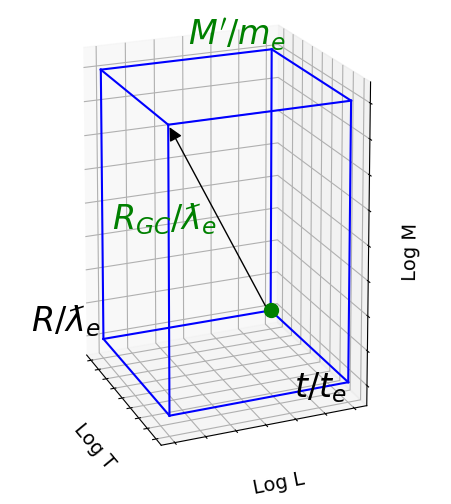
\includegraphics[width=15cm,height=16cm]{./figures/triaxis.png} 
  \caption[Representation Geo dimensionelle du couple Univers-Grandcosmos]{Representation Geo dimensionelle du couple Univers-Grandcosmos. Dans un super espace 3D, les logarithmes naturels de temps, de longueurs et de masses sont consideres comme vecteurs. Le rapport logarithmique du rayon du grand cosmos avec la longueur d'onde de l;electron Compton fait apparaitre un vecteur norme projetant longueur et temps avec une proportion commune; le rayon de Hubble par la longueur d;onde de l'electron Compton et pour le rapport de masse; on considere $M^{\prime}$ par la masse de l'electron. $M^{\prime}$ etant la masse critique dans le Grandcosmos reduit a un hologramme spherique, ceci demontre la confirmation geometrique du principe holographique etendu (2D-1D)applique a l'univers d'entropie de Bekenstein Hawking. L'existence d'un grand cosmos ne peut plus etre niee depuis que la relation entre $e$, $a$ et les logarithmes impliques atteignent une precision de $10^{-7}$.}
  \label{fig:figure_label}
\end{figure}


%\subsection{Lists}
\begin{figure}
  \centering
  %\fbox{\rule[-.5cm]{4cm}{4cm} \rule[-.5cm]{4cm}{0cm}}
  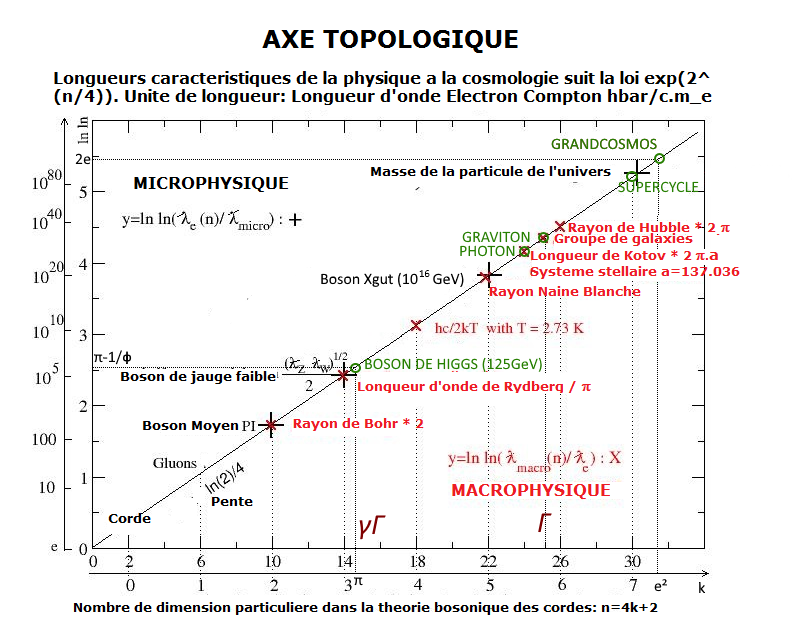
\includegraphics[width=15cm,height=16cm]{./figures/figure.png}
  \caption[Axe Topologique]{L'axe topologique. Le double logarithme naturel (y = lnln(Y)) de quantites physique sans dimensions 
(Y) corresponds a la corde dimensionelle de series n = 4k + 2, de k = 0 a k = 7, montrant la periodicite de Bott qui est a l'origine du nom Axe Topologique.}
  \label{fig:figure_label}
\end{figure}


\end{appendix}
\bibliographystyle{unsrt}  
%\bibliography{references}  %%% Remove comment to use the external .bib file (using bibtex).
%%% and comment out the ``thebibliography'' section.


%%% Comment out this section when you \bibliography{references} is enabled.
\begin{thebibliography}{1}

\bibitem{Sanchez3} Sanchez F.M. ``Towards the grand unified Holic Theory''. Current
Issues in Cosmology. Ed. J.-C. Pecker and J. Narlikar. Cambridge Univ. Press,
2006; p. 257--260.

\bibitem{Sanchez4} Sanchez F; M. ``Holic Principle: The coherence of the Universe`` (Sept 1995), Entelechies, 16th ANPA, 324--344.
\bibitem{Grosmann} Grosmann, M. and Meyrueis P. ``Optics and Photonics Applied to Communication and Processing''. SPIE.  Jan 1979.
\newblock Optics and Photonics Applied to Communication and Processing.
\newblock In {\em SPIE (SPIE), 1979 
  International Conference on}, pages . SPIE, 1979.
\bibitem{Grosmann2} Grosmann, M and Rebordão, José and Meyrueis, Patrick, 1985,02,p761--765,Propagation Of Waves In Optical Systems: Reformulation Of Huyghens Principle For Aspheric Systems,
volume 491, Proceedings of SPIE - The International Society for Optical Engineering, doi:10.1117/12.968010
\bibitem{Kress} Digital Diffractive Optics: An Introduction to Planar Diffractive Optics and Related Technology, by B. Kress, P. Meyrueis, pp. 396. ISBN 0-471-98447-7. Wiley-VCH , October 2000.
\newblock An Introduction to Planar Diffractive Optics and Related Technology.
\bibitem{Sanchez5} F.M. Sanchez, V. Kotov, M. Grosmann, D. Weigel, R. Veysseyre, C. Bizouard, N. Flawisky, D. Gayral, L. Gueroult, Back to Cosmos
\newblock {\em arXiv preprint viXra:1904.0218}, 2019.
\end{thebibliography}
\end{document}
